%\documentclass[tikz, border=5pt]{standalone}
\usetikzlibrary{angles, quotes, shapes.geometric} % 加载角度、引用、直角标记库
\begin{document}
	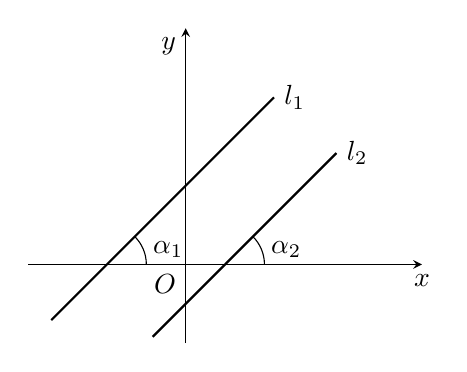
\begin{tikzpicture}[>=stealth, scale=1]
		% 1. 绘制坐标轴
		\draw[->] (-2,0) -- (3,0) node[below] {$x$}; % x轴(带箭头和标签)
		\draw[->] (0,-1) -- (0,3) node[below left] {$y$}; % y轴(带箭头和标签)
		\node at (0,0) [below left] {$O$}; % 原点标记
		
		% 2. 绘制直线 \( l_1 \)(倾斜向上)
		\draw[thick] (-1, 0) --  ++(45: 3) node[right] {$l_1$};
		\draw[thick] (-1, 0) --  ++(-135: 1) ;
		
		% 3. 绘制直线 \( l_2 \)(倾斜向下,与 \( l_1 \) 垂直)
		\draw[thick] (0.5, 0) -- ++(45: 2) node[right] {$l_2$};
		\draw[thick] (0.5, 0) -- ++(-135: 1.3) ;
		
		% 4. 标记角度 \( \alpha_1 \)(\( l_1 \) 与 x 轴正方向的锐角)
		\draw (-0.5, 0) arc (0:45:0.5) node[midway, right ] {$\alpha_1$};
		
		% 5. 标记角度 \( \alpha_2 \)(\( l_2 \) 与 x 轴正方向的角)
		\draw (1, 0) arc (0:45:0.5) node[midway, right ] {$\alpha_2$}; 
		
	\end{tikzpicture}
\end{document}
